% !TEX encoding = UTF-8
% !TEX TS-program = pdflatex
% !TEX root = ../tesi.tex

%**************************************************************
\chapter{Algoritmo per il calcolo della traiettoria}
\label{cap:business-logic}
%**************************************************************

\intro{In questa sezione si documenterà la realizzazione della business logic per il calcolo della traiettoria e l'interfacciamento con il drone.}\\

%**************************************************************

\section{Strumenti utilizzati}
Il linguaggio scelto per sviluppare questa componente della Proof of Concept è Java nella versione 11. Si è usato l'IDE IntelliJ IDEA Education, il quale offre un ambiente di sviluppo integrato sia per Java che per Python. In questo modo è stato possibile eseguire il server per le predizioni insieme al modulo del programma in Java che si interfaccia con questo in modo molto semplificato.

\section{Architettura generale}
L'architettura data all'applicazione è quella del monolite a strati, di cui si può vedere una rappresentazione ad alto livello nella figura \ref{fig:layered_architecture}.

\subsection{Strato di persistenza}
Nel nostro caso al posto del Database, alla base, c'è il server che espone la rete neurale per le predizioni. Di conseguenza lo strato di persistenza è l'insieme di quelle classi addette a comporre la richiesta HTTP da inviare all'end-point, le quali sono collocate nel package prediction. In particolare all'interno di questo troviamo la classe NeuralNetworkClient che contiene

\begin{figure}
    \centering
    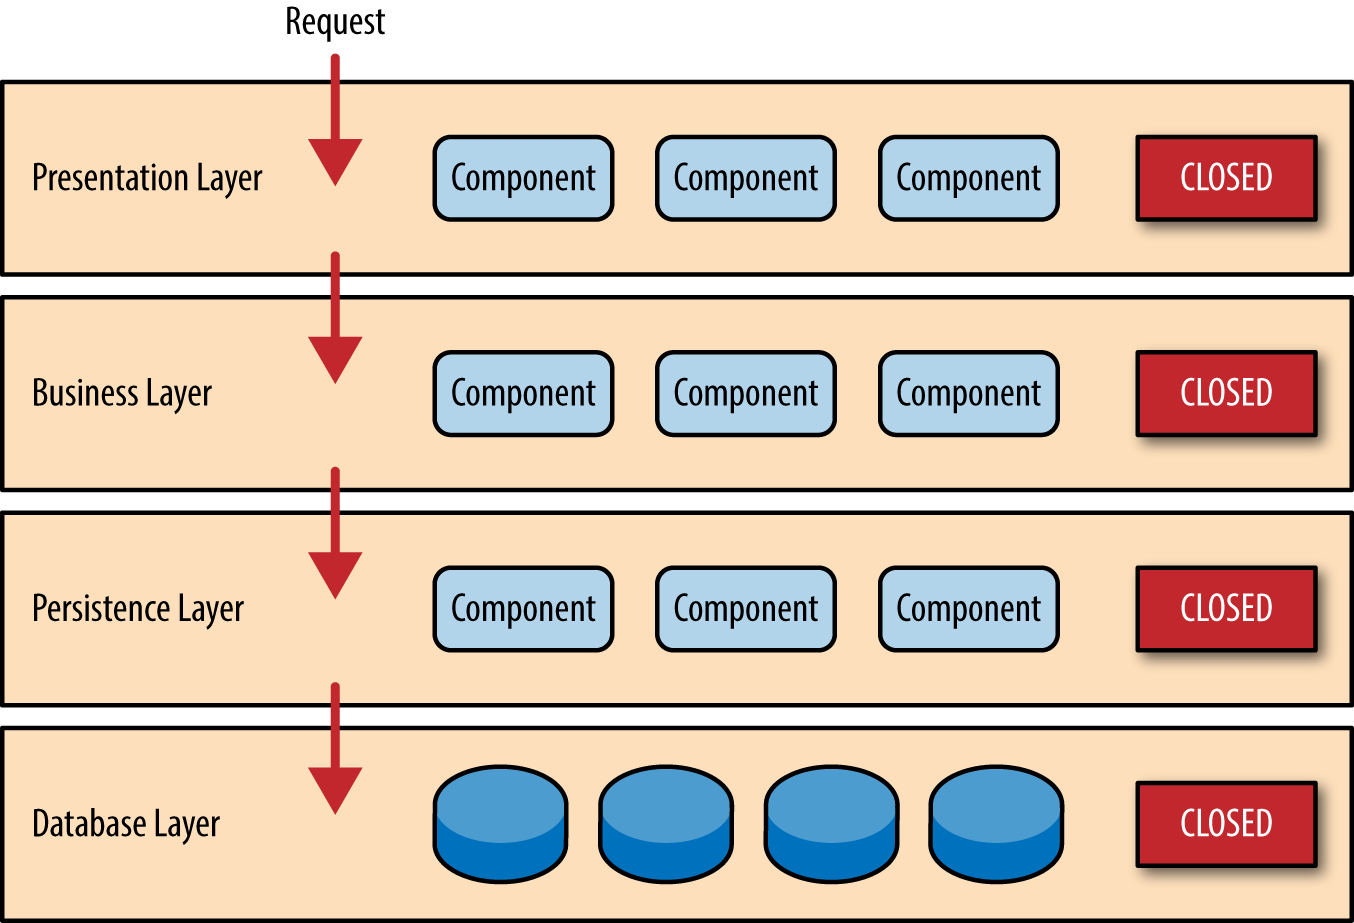
\includegraphics[width=\textwidth]{immagini/layered_archiecture.png}
    \caption{Architettura monolitica a strati}
    \label{fig:layered_architecture}
\end{figure}